\section{Improving the robustness to rain}
\label{sec:improving}

We now wish to demonstrate the usefulness of our rain rendering pipeline for improving robustness to rain through extensive evaluations on synthetic and real rain databases. For the sake of coherence, the improvements are shown on the same tasks, algorithms, and test data from sec.~\ref{sec:real_data}.

\subsection{Training methodology}

While the ultimate goal is to improve robustness to rain, we aim at training a single model which performs well across a wide variety of rainfall rates (including clear weather). Having a single model is beneficial over employing, e.g., intensity-specific encoders~\cite{porav2019can}, since it removes the need for determining rain intensity from the input image. 
Because rain significantly alters the appearance of the scene, we found that training from scratch with heavy rain or random rainfall rates fails to converge.
Instead, we refine our \textit{untuned} models using curriculum learning~\cite{bengio2009curriculum} on rain intensity in ascending order (25, then 50, and finally 100mm/hr rain). The final model is referred as \textit{finetuned} and is evaluated against various weather conditions. Note that, for hybrid augmentation finetuning, the curriculum starts with the refinement on GAN images first and then go through the ascending rain intensities. The same images are used for all steps of the curriculum.

In order to avoid training and testing on the same set of images, in this section, we further divide the nuScenes-augment into train/test subsets of 1000 images each (ensuring they are taken from different scenes). 
Each algorithm is thus refined on the 1000 images from nuScenes-augment(train), and undergo a specific training process. For object detection, YOLOv2~\cite{redmon2017yolo9000} is trained each step at a learning rate of $0.0001$ and a momentum of 0.9 for 10 epochs with a burn-in of 5 epochs. For semantic segmentation, PSPNet~\cite{zhao2017pspnet} is trained with a learning rate of $0.0004$ and a momentum of 0.9 for 10 epochs. Finally, for depth estimation, Monodepth2~\cite{godard2019digging} is trained on triplets of consecutive images using a learning rate of $0.00001$ with the Adam optimizer for 10 epochs with $\beta = \left\{ 0.5, 0.999 \right\}$.  

\subsection{Improvement on synthetic rain}
\label{sec:perf_synth_data}

The synthetic evaluation is conducted on the set of 1000 images from nuScenes-augment(test), with rain up to 200mm/hr. Note again, for our hybrid GAN+PBR, 0mm/hr of rain correspond to the GAN-only augmented results.

Fig.~\ref{fig:synth_eval} shows the performance of our untuned and finetuned model for the three vision tasks on different augmented dataset. Fig.~\ref{fig:synth_eval_obj} and fig.~\ref{fig:synth_eval_depth} are for object detection (YOLOv2~\cite{redmon2017yolo9000}) and depth estimation (Monodepth2~\cite{godard2019digging}) on nuScenes-clear augmented data while fig.~\ref{fig:synth_eval_segm} is for the semantic segmentation (PSPNet~\cite{zhao2017pspnet}) on Cityscapes. We observe a significant improvement in both tasks and additional increase in robustness even in clear weather when refined using our augmented rain. Of interest, we also improve at the unseen 200mm/hr rain though the network was only trained with rain up to 100mm/hr.
The intuition here is that when facing adverse weather, the network learns to focus on strongest relevant features for all tasks and thus gain robustness. 

\paragraph{PBR.} For YOLOv2, the finetuned detection performance stays higher than its clear untuned counterpart in the 0-200mm/hr interval. Explicitly, it goes from 34.5\% to 31.0\% whereas the untuned model starts at 34.6\% and finishes at 20.4\%. For PSPNet, the segmentation exhibits a significative improvement when refined although at 100mm/hr the model is not fully able to compensate the effect of rain and drops to 54.0\% versus 52.0\% when untuned. Monodepth2 finetuning helps only for higher rain intensity level (+25mm/hr) and the error differences between 100mm/hr and 200mm/hr stay in the same ballpark (\textasciitilde{}1.2\%). This makes sense considering that since the occlusion created by rain streaks is minimum with a low rain intensity, the untuned model would not be strongly affected.

\paragraph{GAN+PBR.} In the case of YOLOv2, we notice a major difference between the hybrid  GAN+PBR untuned and finetuned performances. Indeed, the hybrid finetuned performance at 100mm/hr is at 21.7\% and only at a measly 7.5\% for the untuned model. The same goes for Monodepth2 for hybrid images performance with 5.7\% and 8.9\% at 100mm/hr for finetuned and untuned respectively. 
It is interesting to note that, for all tasks, performance evaluated on finetuned hybrid image decrease slower than for untuned models. This demonstrates again that more robust models are learned when finetuning with our rain translations.

\begin{figure}
 \centering
 \subfloat[Object detection~\cite{redmon2017yolo9000}]{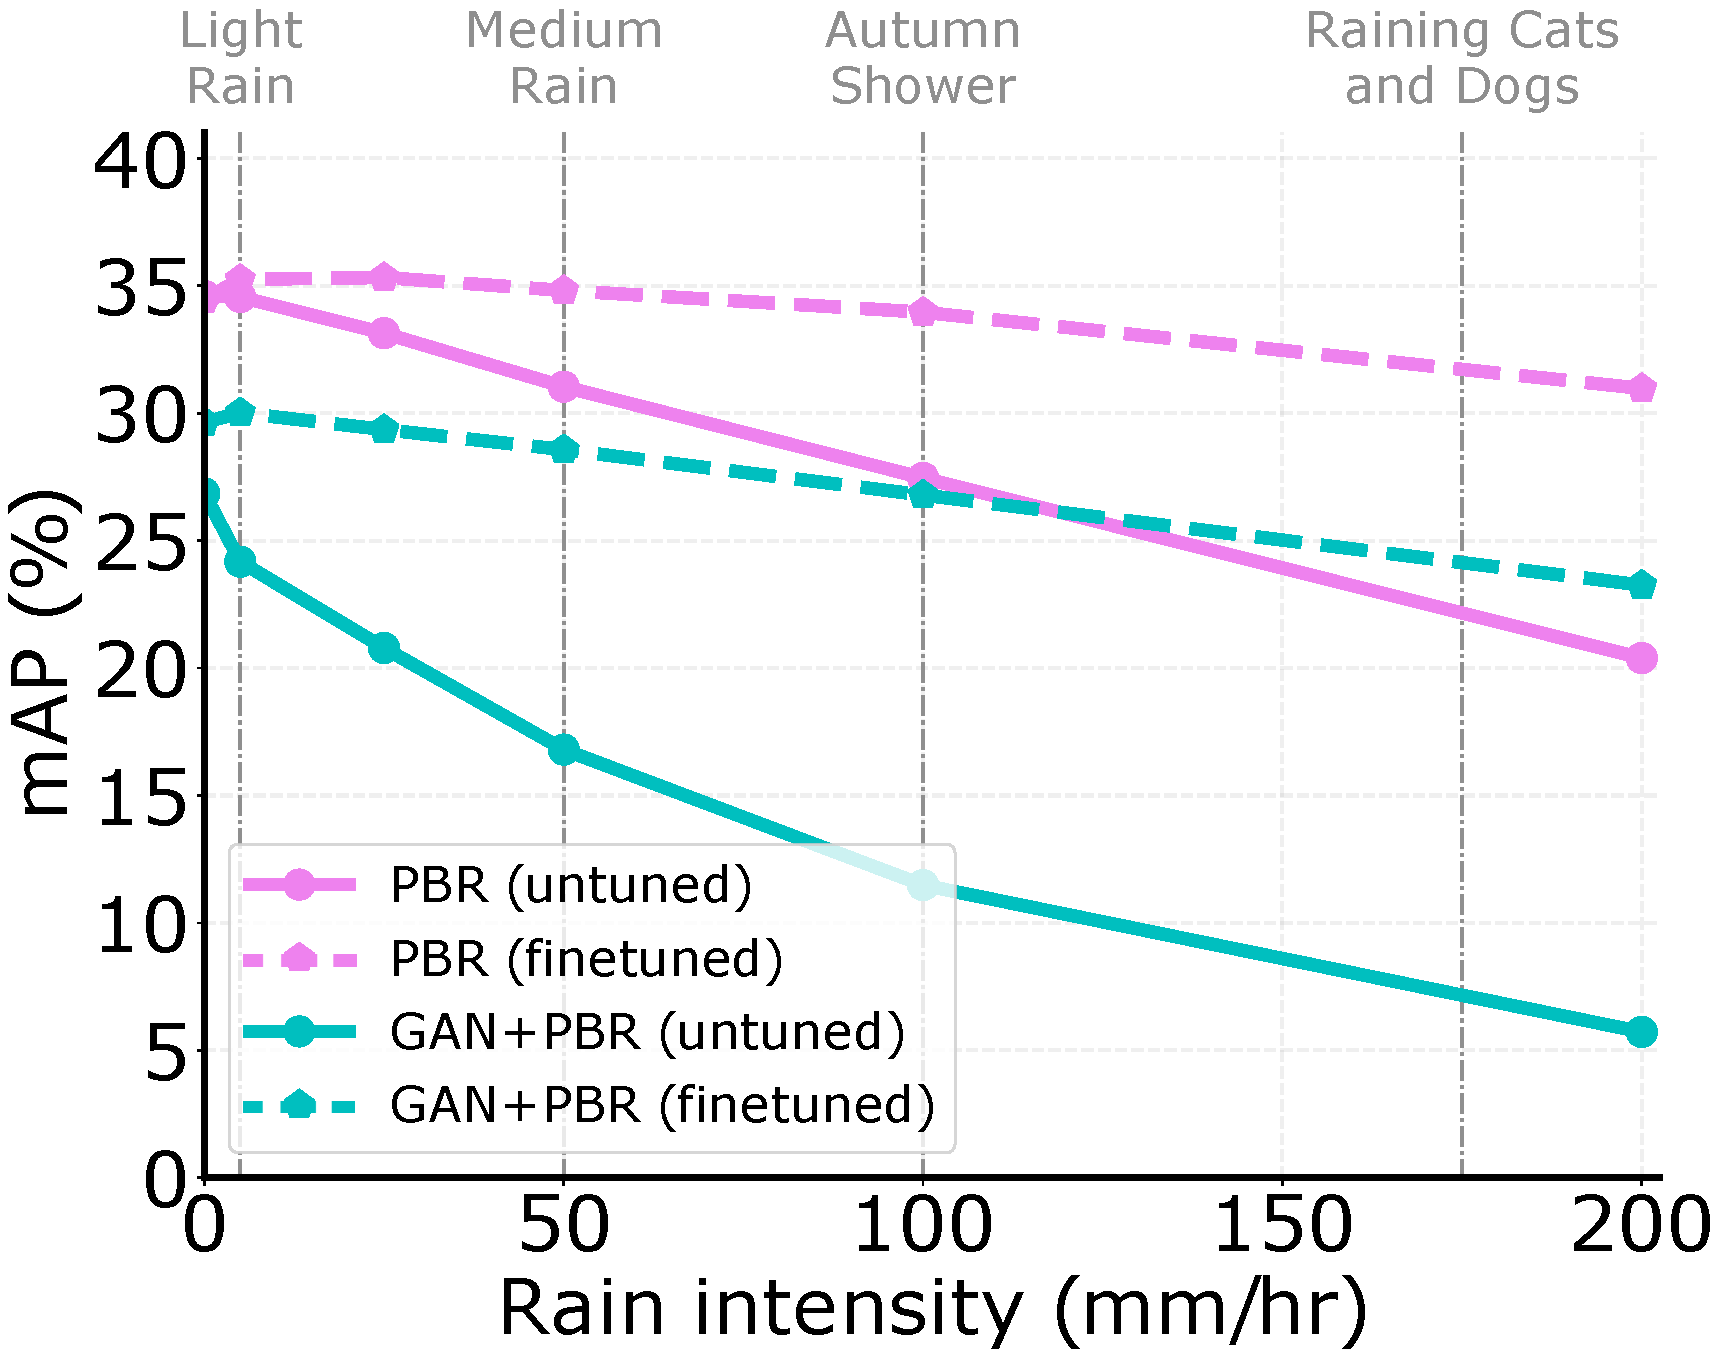
\includegraphics[width=0.485\linewidth]{figures/plots/yolov2_synth_performances.pdf}\label{fig:synth_eval_obj}} \hfill%
 \subfloat[Depth estimation~\cite{godard2019digging}]{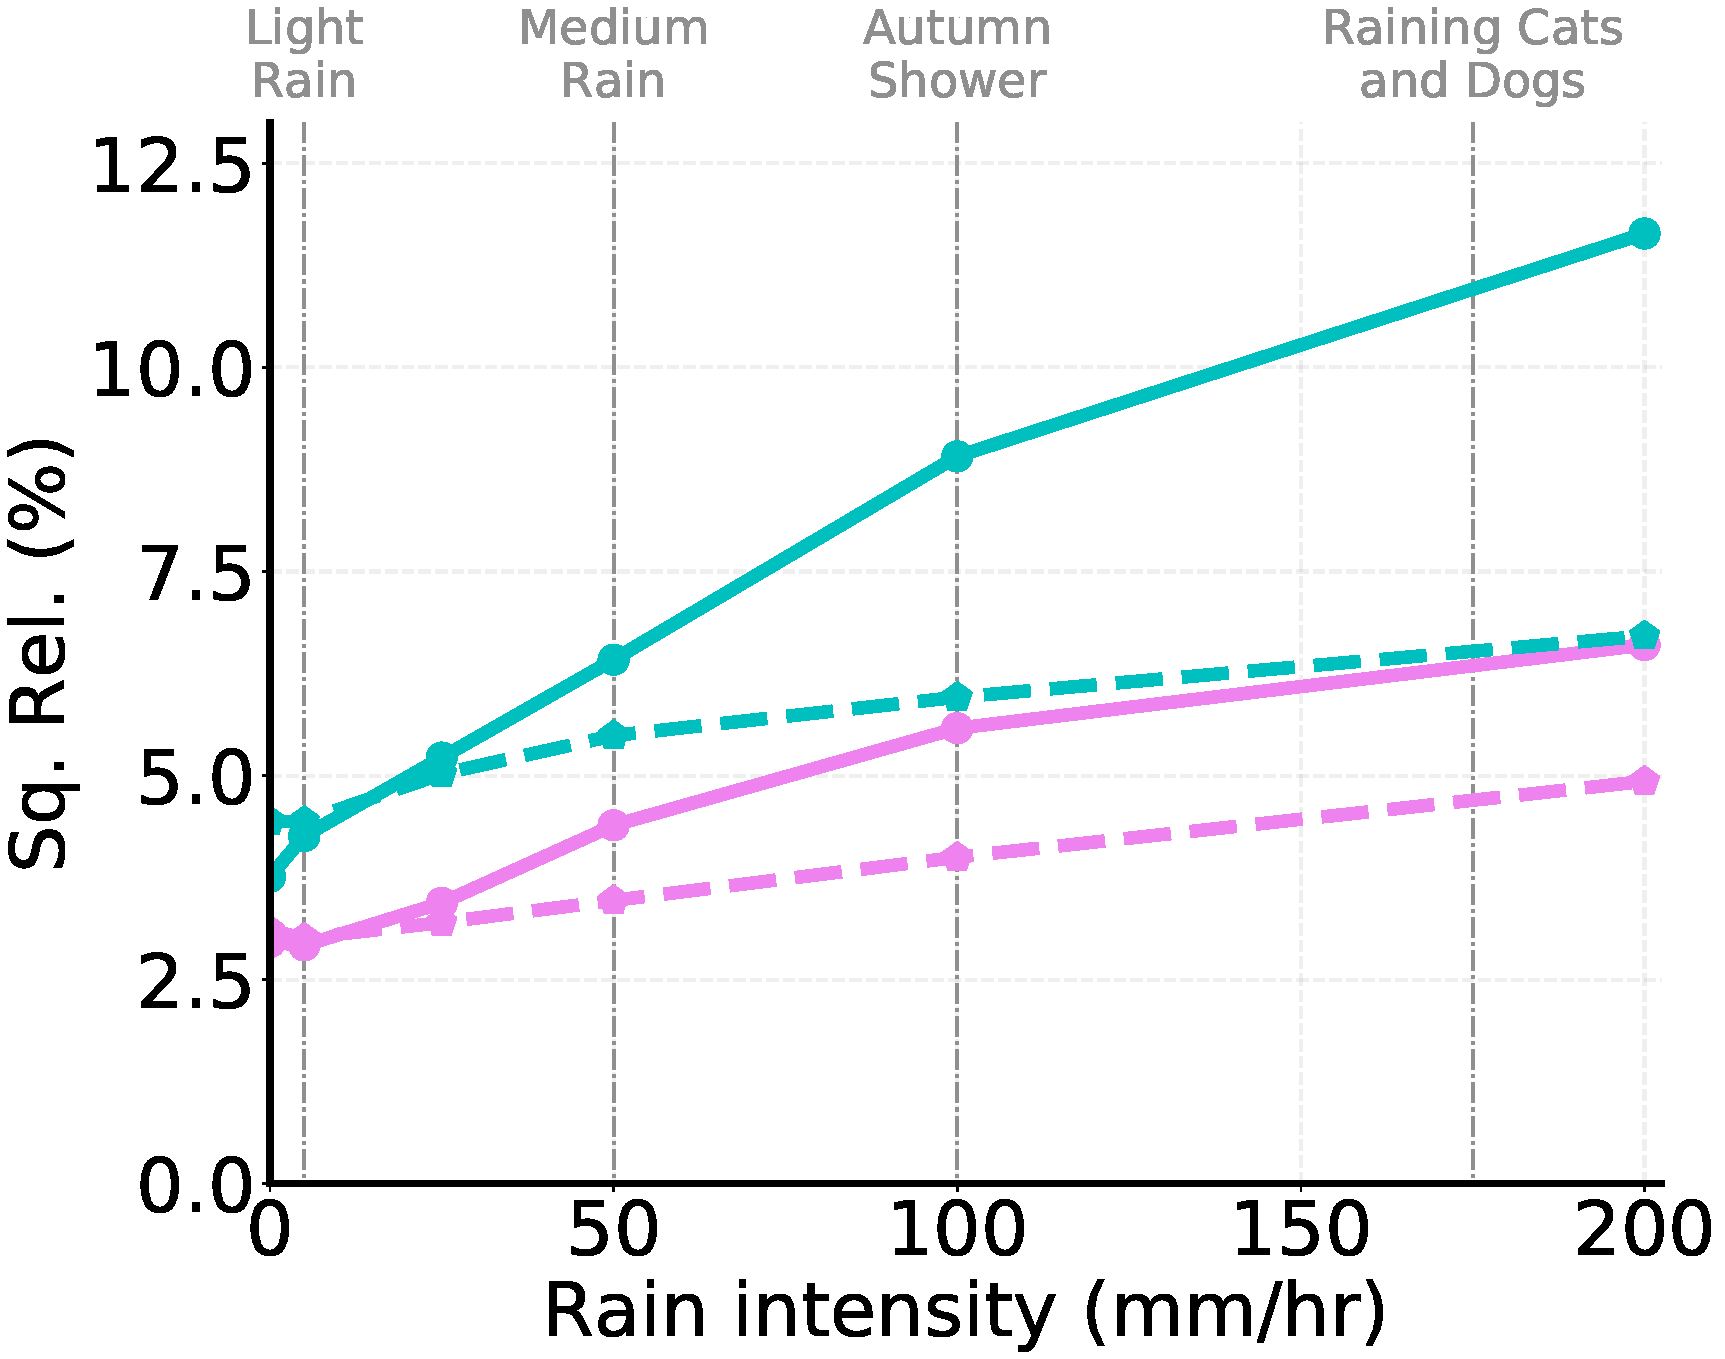
\includegraphics[width=0.485\linewidth]{figures/plots/monodepth2_synth_performances.pdf}\label{fig:synth_eval_depth}} 
 
 \subfloat[Semantic segmentation~\cite{zhao2017pspnet}]{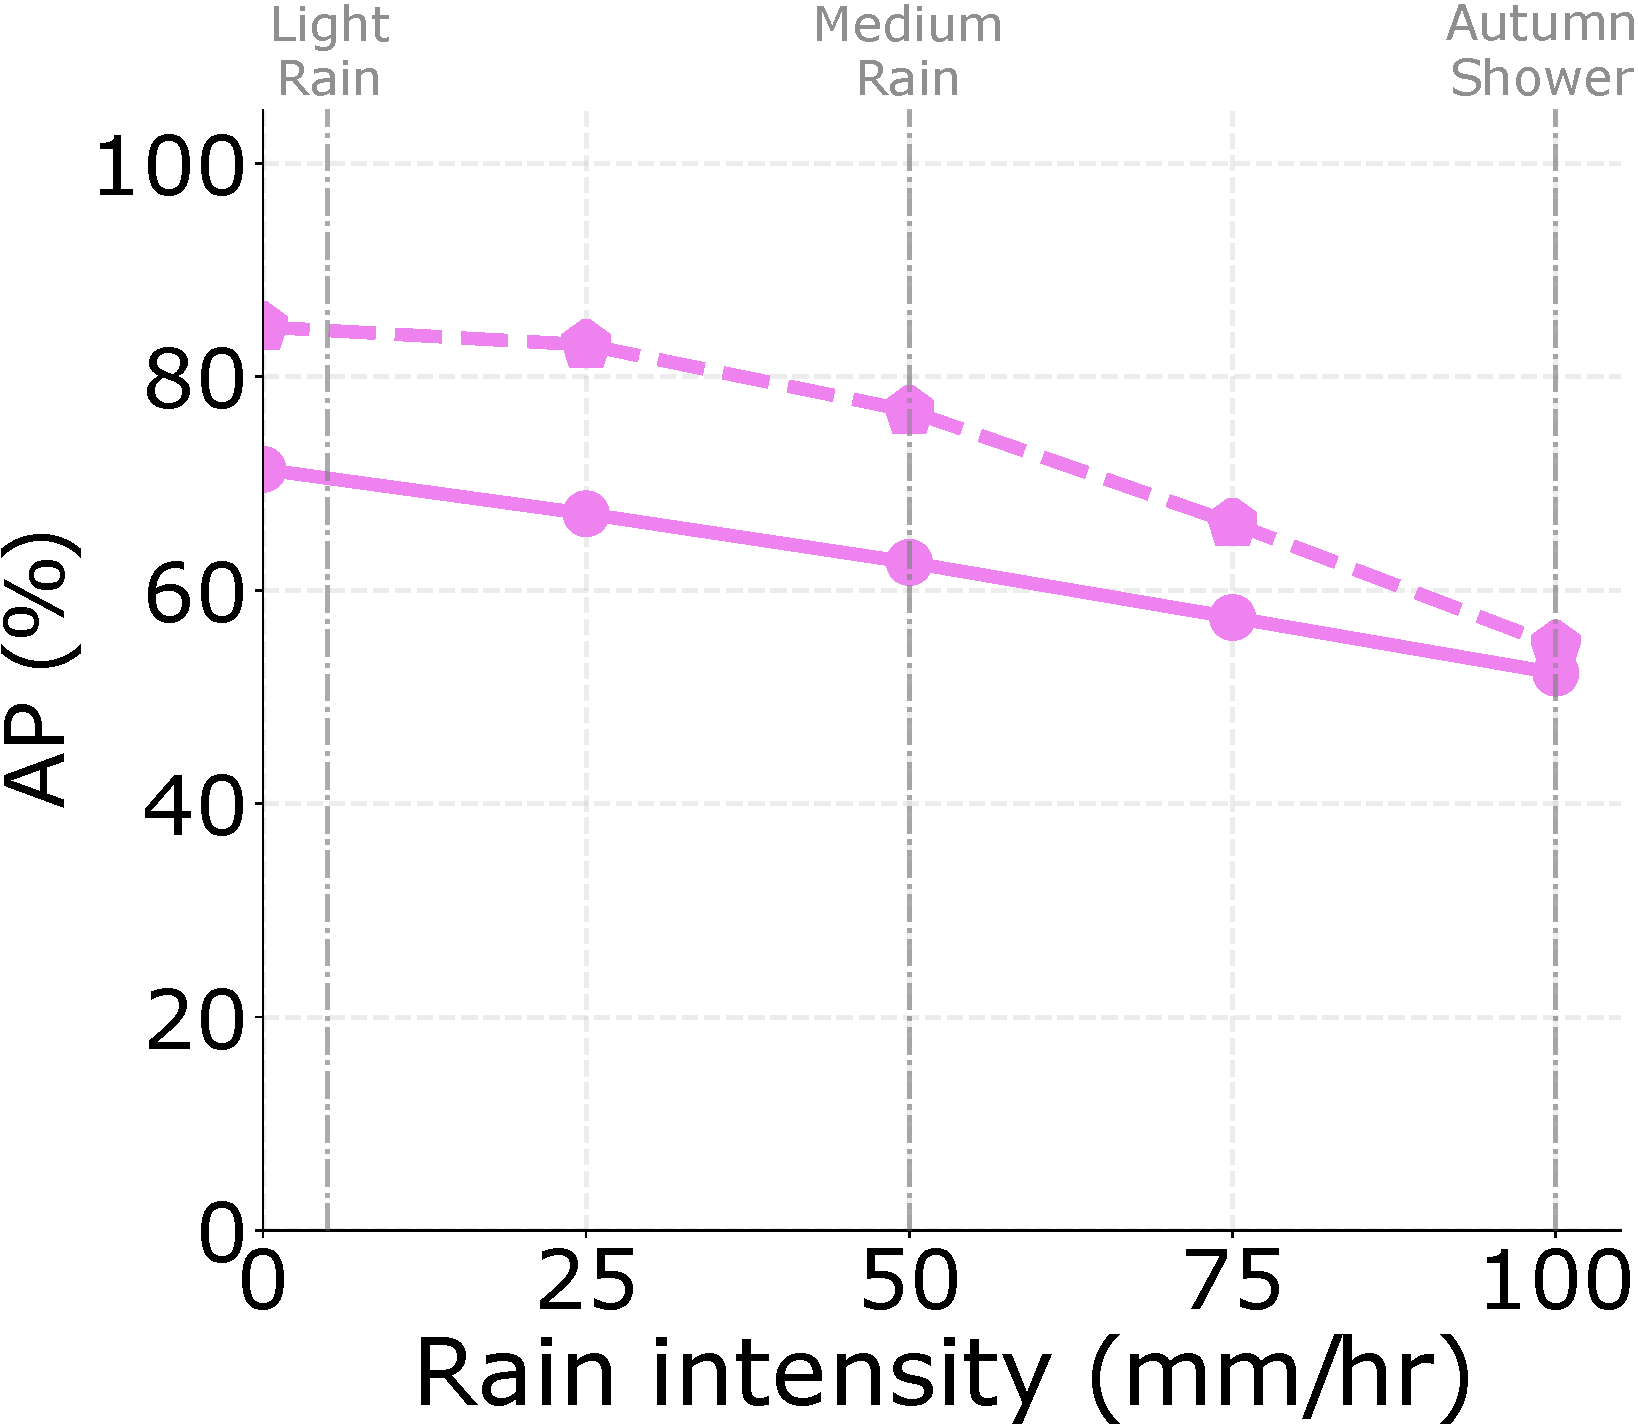
\includegraphics[width=0.485\linewidth]{figures/plots/pspnet_synth_performances.pdf}\label{fig:synth_eval_segm}}
 \caption{\textbf{Original (untuned) or finetuned performance on rain-augmented versions of nuScenes~\protect\subref{fig:synth_eval_obj}-\protect\subref{fig:synth_eval_depth} and Cityscapes~\protect\subref{fig:synth_eval_segm}.} Not only the finetuned models significantly outperform untuned models, but they exhibit a lower decrease with rain intensity, demonstrating increased robustness to both rain and clear weather.}
 \label{fig:synth_eval}
\end{figure}

\subsection{Improvement on real rain}
\label{sec:perf_real_data}

We evaluate the performance on real rain, using our nuScenes-rain(test) subset of images (see sec.~\ref{sec:real_data}).
Table~\ref{tab:impr_finetune} shows that our finetuning leads to performance increase in real rainy scenes compared to untuned performance in rain. We note for object detection (PBR: +20.7\%, GAN: +10.9\%, GAN+PBR: +21.0\%), for semantic segmentation (PBR: +36.9\%), and for depth estimation (PBR: 0.0\%, GAN: +3.8\%, GAN+PBR: +8.2\%) tasks. 
In clear weather, our finetuned model performs on par with the untuned version, sometimes even better. This boost in performance could be seen as the network learning to rely on more robust features, somehow invariant to rain streaks. 

Depth estimation underperformance for PBR finetuning can be explained by the learning loss of Monodepth2 which is, in short, a reprojection error which would not fare well with rain streaks as they do not reproject in consecutive frames. 
Interestingly, this problem does not seem to affect the GAN or GAN+PBR finetuned model, possibly because the GAN is being trained on split of nuScenes subsequently leading to finetuning images that are more resembling of the test set.
These results demonstrate the usefulness of our different rain rendering frameworks for real rain scenarios.

\begin{table}
 \centering
 \scriptsize
 \setlength{\tabcolsep}{0.125cm}
 \renewcommand{\arraystretch}{1.25}
 \stackunder[2pt]{\begin{tabular}{lcccccc}
  \toprule
  & \multicolumn{2}{c}{Object det. \cite{redmon2017yolo9000}} & \multicolumn{2}{c}{Semantic seg. \cite{zhao2017pspnet}} & \multicolumn{2}{c}{Depth est. \cite{godard2019digging}} \\
  & \multicolumn{2}{c}{\tiny{mAP (\%) $\uparrow$}} & \multicolumn{2}{c}{\tiny{AP (\%) $\uparrow$}} & \multicolumn{2}{c}{\tiny{Sq. err. (\%) $\downarrow$}} \\ 
  \cmidrule(lr){2-3}\cmidrule(lr){4-5}\cmidrule(lr){6-7}
  & Clear & Rain & Clear & Rain & Clear & Rain \\
  \midrule
  Untuned & 32.53 & 16.30 & \textbf{40.8} & 18.7 & 2.96 & 3.53 \\
  Finetuned \tiny{(PBR)} & \textbf{33.51} & 19.68 & 39.0 & \textbf{25.6} & 3.15 & 3.54 \\
  Finetuned \tiny{(GAN)} & 32.26 & 18.07 & * & * & \textbf{2.89} & 3.40 \\
  Finetuned \tiny{(GAN+PBR)} & 30.59 & \textbf{19.73} & * & * & 3.01 & \textbf{3.29} \\ 
  \midrule
  De-rained \tiny{DualResNet} & 32.60 & 18.30 & * & * & 2.25 & 3.09 \\
  \bottomrule
 \end{tabular}}{* Not evaluated due to lack of semantic labels for GAN training.}
 \vspace{.5em}
 \caption{\textbf{Improving performance of computer vision tasks on real nuScenes~\cite{caesar2019nuscenes} images.} These tasks are object detection (YOLOv2~\cite{redmon2017yolo9000}), semantic segmentation (PSPNet~\cite{zhao2017pspnet}), and depth estimation (Monodepth2~\cite{godard2019digging}). The last line shows performance with the untuned models after the de-raining~\cite{liu2019dual} process.}
 \label{tab:impr_finetune}
\end{table}

\subsection{De-raining comparison}
\label{sec:deraining}

We now compare to the strategy of de-raining images first and then running un-tuned vision algorithms. To this end, we used the state-of-the-art de-raining method DualResNet~\cite{liu2019dual}, finetuned using nuScenes-clear augmented with GAN+PBR to accommodate for the domain gap.

During the de-raining fine-tuning process, random batches of $\left\{25, 50, 100, 200\right\}$mm/hr paired with their non-augmented counterpart are generated. Except for a smaller learning rate ($10^{-5}$), we used the DualResNet default hyper-parameters (Adam optimizer, batch and crop size of 40 and 64 respectively).

With this de-raining finetuned model, we compare the performance of our ``untuned'' object detection (YOLOv2~\cite{redmon2017yolo9000}) and depth estimation (Monodepth2~\cite{godard2019digging}) models. Fig.~\ref{fig:deraining_synth_perf} shows the performance of the de-raining strategy compared to our ``rain-aware'' GAN+PBR finetuned models. Here, we observe that the rain-aware models offer improved performance for object detection over de-raining, while the latter improves depth estimation. This is likely due to the fact that streaks occlude the scene background, while de-raining acts as prior impainting thus easing depth estimation.

We also applied the same de-raining strategy to the real nuScenes images and report performance in the last row of table~\ref{tab:impr_finetune}. Again, for object detection on rainy images our rain-aware models perform better than de-raining. However, for depth estimation, the de-raining strategy is better for both clear and rainy images. This is consistent with the results obtained on synthetic data.

These experiments illustrate that de-raining is also a valid strategy that may even outperform ``rain-aware'' algorithms. However, this comes at the cost of having to perform two tasks, which may limit practical applications. On the long term, we believe rain-robust algorithms offer an exciting new research paradigm while avoiding the in-filling of occluded areas.

\begin{figure}
 \centering
 \subfloat[Object detection~\cite{redmon2017yolo9000}]{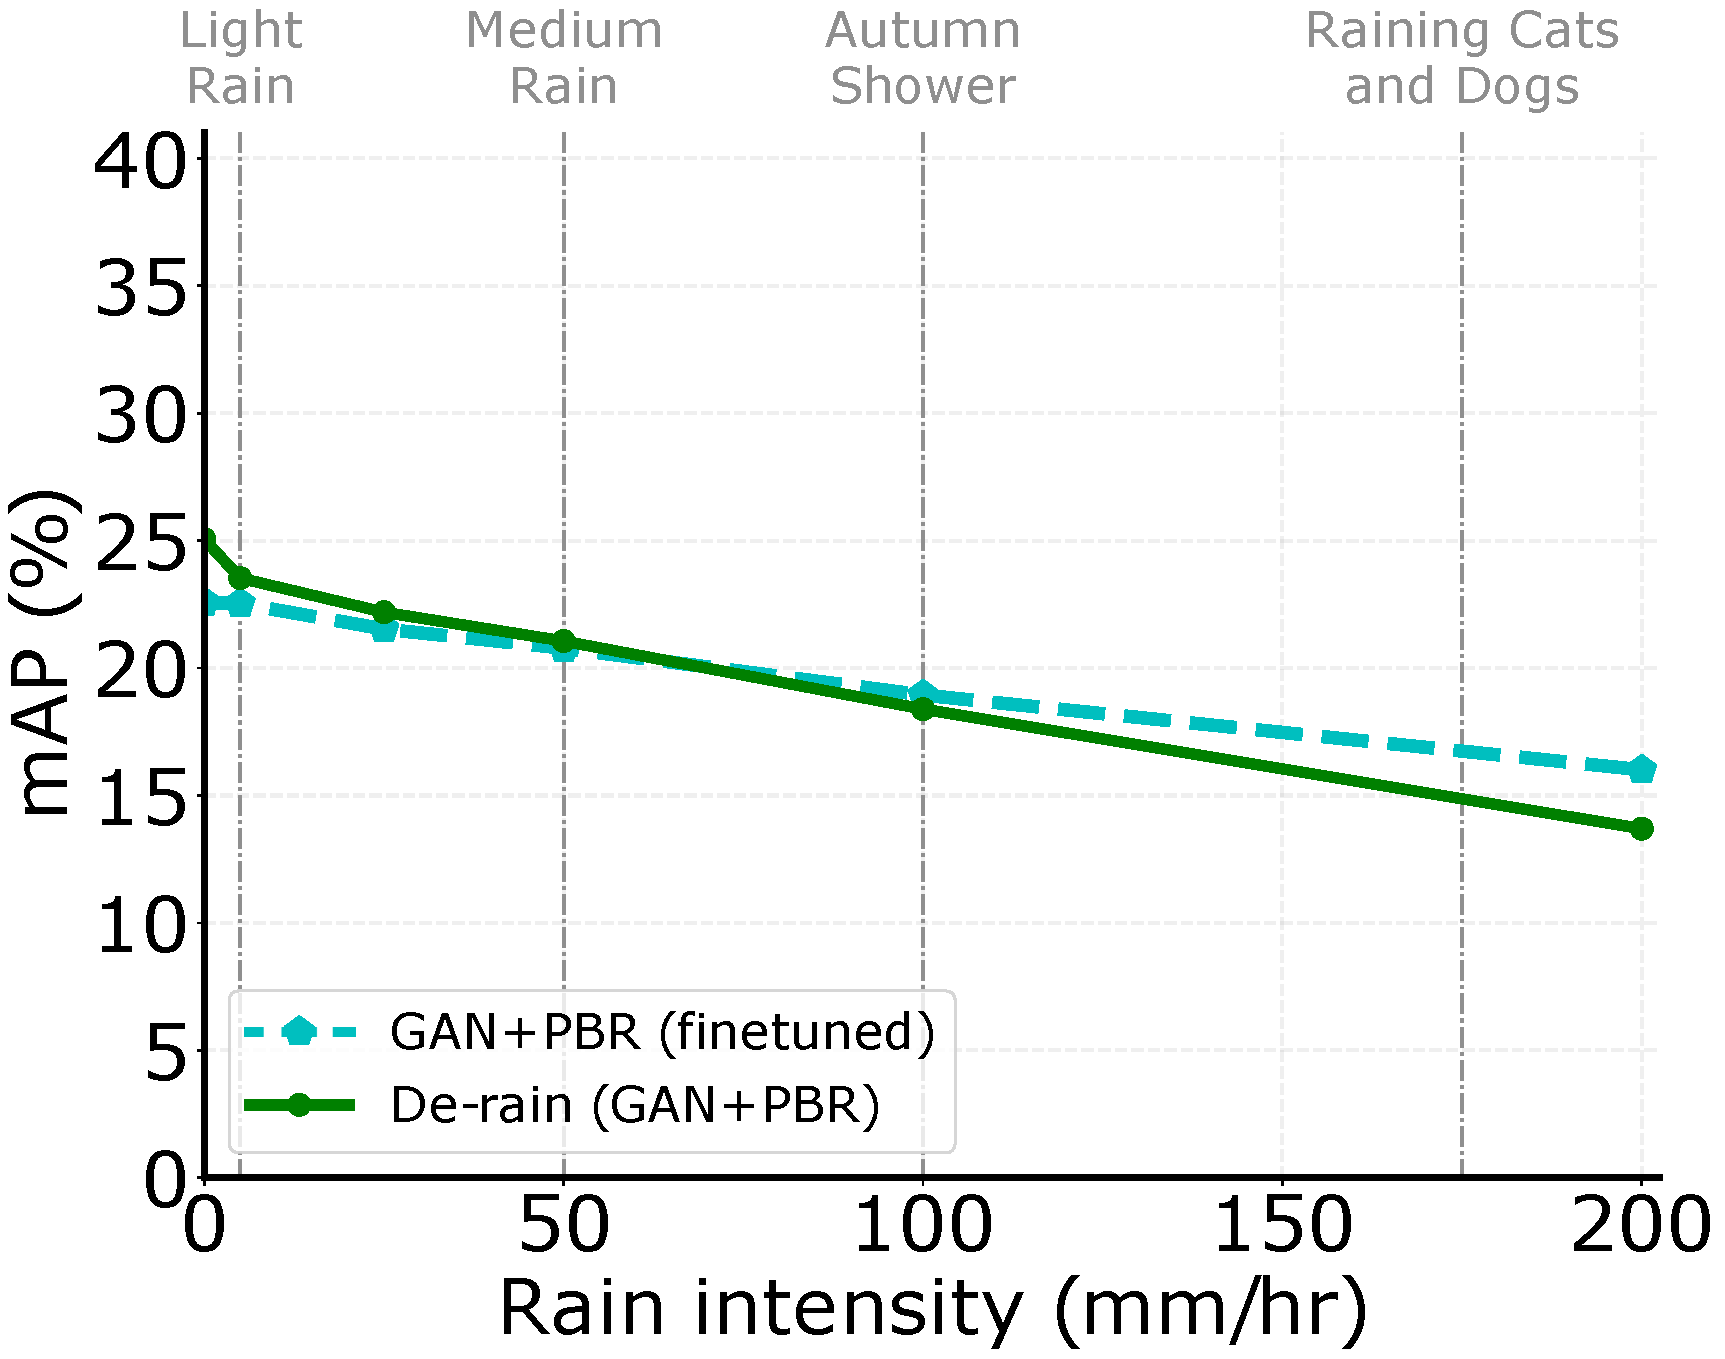
\includegraphics[width=0.485\linewidth]{figures/plots/yolov2_derain_performances.pdf} \label{fig:derain_obj_detect_perf}} \hfill%
    \subfloat[Depth estimation~\cite{godard2019digging}]{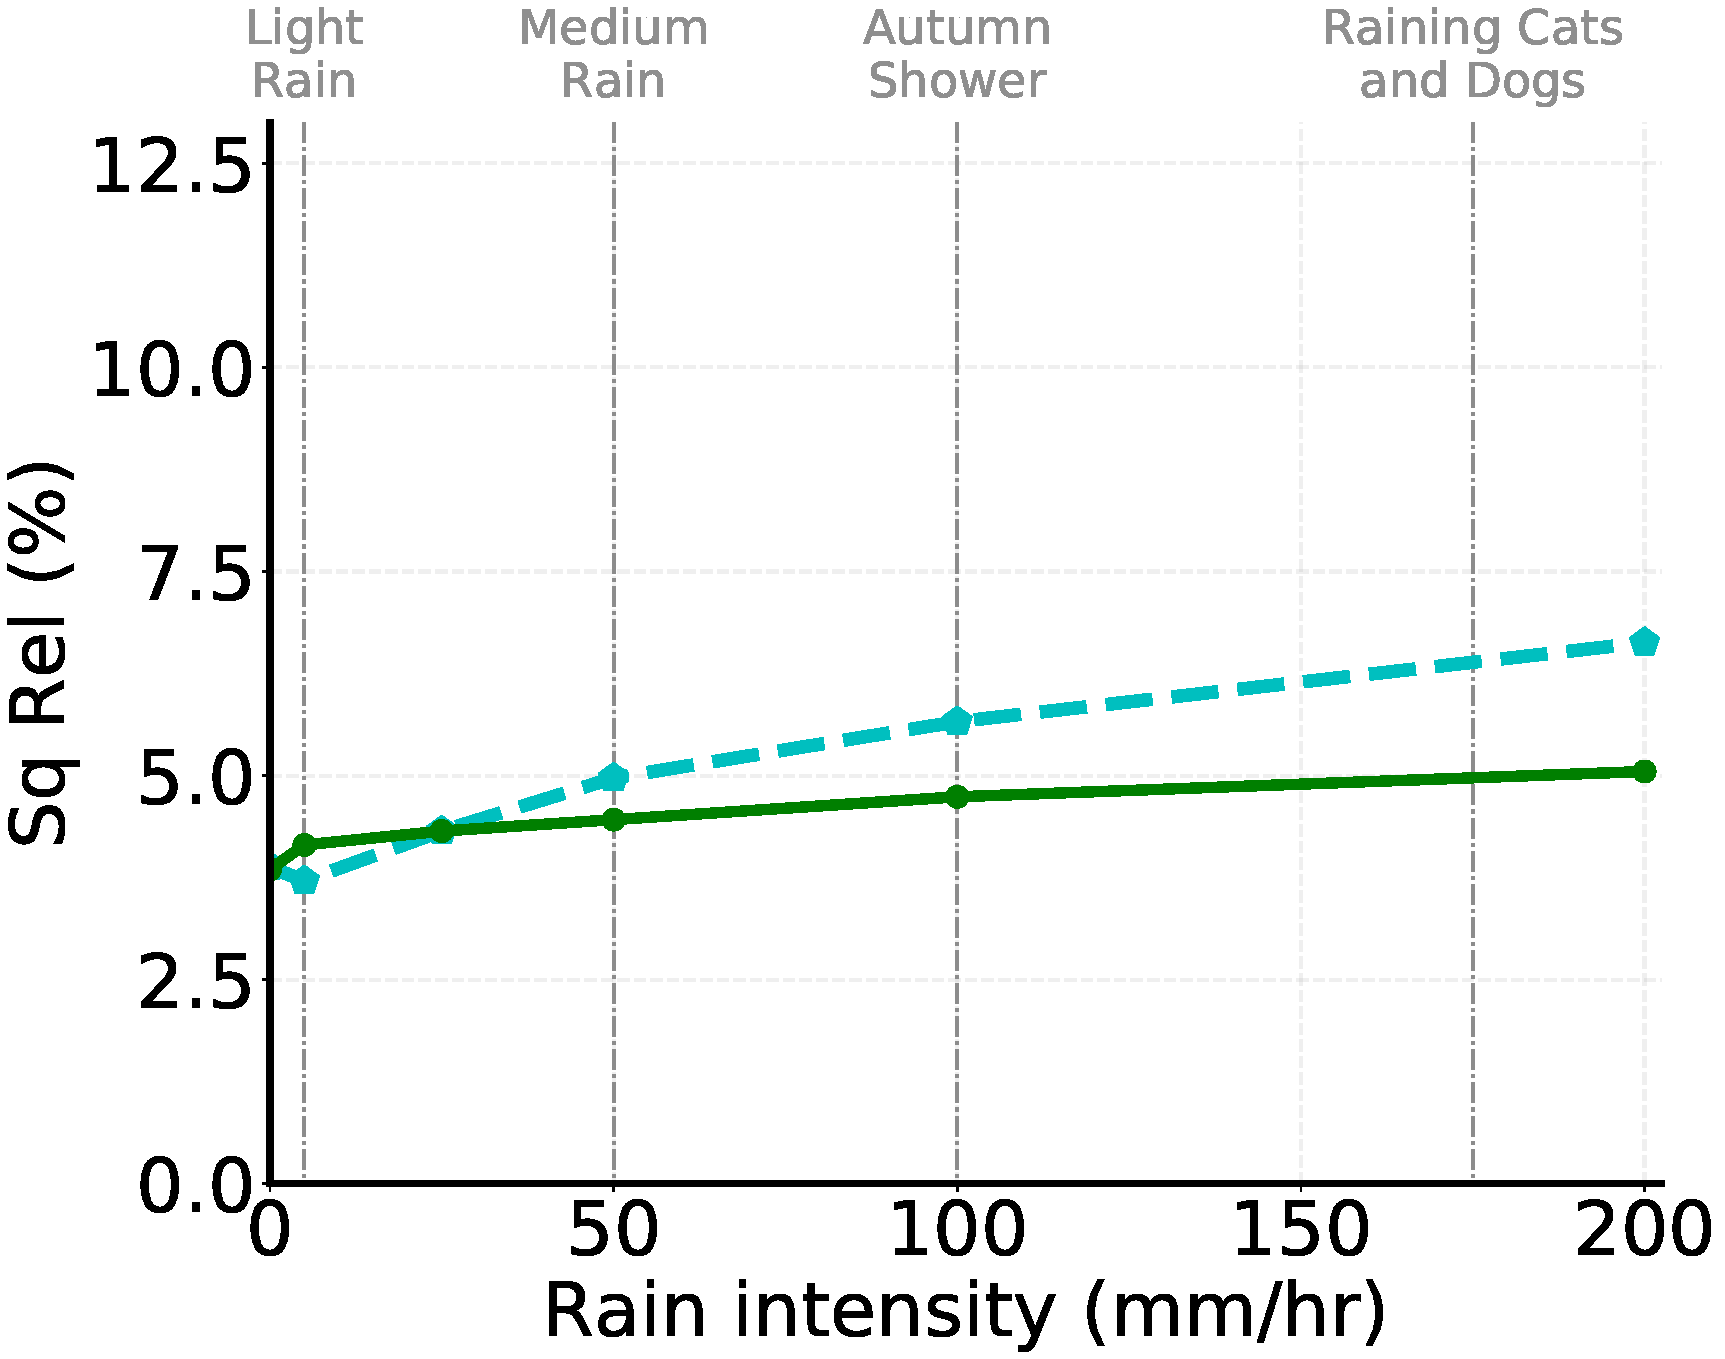
\includegraphics[width=0.485\linewidth]{figures/plots/monodepth2_derain_performances.pdf} \label{fig:derain_depth_estim_perf}} 
 \caption{\textbf{Performance with varying rain intensities on de-rained GAN+PBR synthetic images.} The de-raining is performed with \cite{liu2019dual}. We see that the performance on both tasks decrease linearly for both \protect\subref{fig:derain_obj_detect_perf} object detection with YOLOv2~\cite{redmon2017yolo9000} and \protect\subref{fig:derain_depth_estim_perf} depth estimation with Monodepth2~\cite{godard2019digging}. Performance on both tasks are lower at low rain intensities (and the opposite at high rain intensities) compared to models finetuned with GAN+PBR synthetic images (cf. fig.~\ref{fig:synth_eval}).}
 \label{fig:deraining_synth_perf}
\end{figure}


